\newpage
\subsection{Artificial Neural Networks}
Artificial Neural Networks (ANNs) are function approximators loosely inspired by nervous systems.
ANNs consist of nodes, also called neurons, connected by directed links (see Figure \ref{feedforward}). 
A node is either an input node that receives external input data, an output node which sends out a final value computed
by the network or a hidden node, a node that exists somewhere between the input and output nodes. Each node receives signals, either
as the initial input or as signals from other nodes. Each link is associated with a weight which inhibits or excites the signal 
passing over it. The nodes sum the incoming weighted signals, calculating a net input signal. A function is applied to the net input 
signal to generate an output signal (see Figure \ref{neuron}). The function is referred to as an activation function and regulates the strength of the output 
signal given the net input signal. The signal is propagated through the network until it reaches the final output node or nodes.


\begin{figure}[htb]
    \begin{mdframed}
        \begin{subfigure}[b]{0.5\textwidth}
            \centering
            \resizebox{0.7\textwidth}{!}{\def\layersep{2.5cm}

\begin{tikzpicture}[shorten >=1pt,->,draw=black!50, node distance=\layersep]
    \tikzstyle{every pin edge}=[<-,shorten <=1pt]
    \tikzstyle{neuron}=[circle,fill=black!25,minimum size=17pt,inner sep=0pt]
    \tikzstyle{input neuron}=[neuron, fill=green!50];
    \tikzstyle{output neuron}=[neuron, fill=red!50];
    \tikzstyle{hidden neuron}=[neuron, fill=blue!50];
    \tikzstyle{bias neuron}=[neuron, fill=yellow!50];
    \tikzstyle{annot} = [text width=4em, text centered]

    % Draw the input layer nodes.
    \foreach \name / \y in {1,...,3}
        \node[input neuron] (I-\name) at (0,-\y) {};

    % Draw the hidden layer nodes.
    \foreach \name / \y in {1,...,4}
        \path[yshift=0.5cm]
            node[hidden neuron] (H-\name) at (\layersep,-\y cm) {};

    % Draw the output layer nodes
    \node[output neuron,pin={[pin edge={->}]right:}, right of=H-2] (O-1) {};
    \node[output neuron,pin={[pin edge={->}]right:}, right of=H-3] (O-2) {};

    % Connect input layer with hidden layer.
    \foreach \source in {1,...,3}
        \foreach \dest in {1,...,4}
            \path (I-\source) edge (H-\dest);

    % Connect hidden layer with output layer.
    \foreach \source in {1,...,4}
        \path (H-\source) edge (O-1);

    \foreach \source in {1,...,4}
        \path (H-\source) edge (O-2);


    % Higlight path
    \foreach \source in {1,...,3}
        \draw[->,line width=0.4mm] (I-\source)--(H-1) node[pos=.6,above]{};

    \foreach \dest in {1,...,2}
        \draw[->,line width=0.4mm] (H-1)--(O-\dest) node[pos=.6,above]{};
    % Annotate the layers.
    %\node[annot,above of=H-1, node distance=0.65cm] (hl) {Hidden};
    %\node[annot,left of=hl] {Inputs};
    %\node[annot,right of=hl] {Outputs};
\end{tikzpicture}}
            \caption{ANN example.}
            \label{feedforward}
        \end{subfigure}
        \begin{subfigure}[b]{0.5\textwidth}
            \centering
            \resizebox{0.9\textwidth}{!}{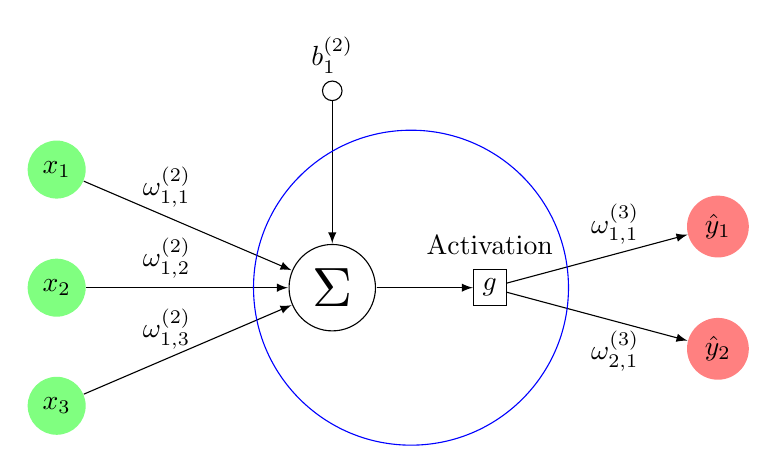
\begin{tikzpicture}[>=latex]
    \path
    % Summation
    (0,0)     node[circle,draw,scale=2,inner sep=2pt] (summation) {$\Sigma$}

    % Bias node
    +(90:2.5) node[circle,draw,inner sep=2.5pt] (bias) {}
              node[above=1mm] {$b_1^{(2)}$}
    % Input nodes
    +(-3.5,1.5)  node[circle,fill=green!50]  (input1) {$x_1$}
    +(-3.5,0)    node[circle,fill=green!50]  (input2) {$x_2$}
    +(-3.5,-1.5) node[circle,fill=green!50]  (input3) {$x_3$}

    % Activation function
    (2,0)    node[draw] (activation) {$g$} node[above=3mm]{Activation}

    % Output nodes
    +(15:3)  node[circle,fill=red!50]  (output1) {$\hat{y}_1$}
    +(-15:3) node[circle,fill=red!50]  (output2) {$\hat{y}_2$};

    % Link the different parts of the graph
    \draw[->] (summation)--(activation);
    \draw[->] (bias)--(summation);
    \draw[->] (activation)--(output1) node[pos=.6,above]{$\omega_{1,1}^{(3)}$};
    \draw[->] (activation)--(output2) node[pos=.6,below]{$\omega_{2,1}^{(3)}$};
    \draw[->] (input1)--(summation) node[pos=.4,above]{$\omega_{1,1}^{(2)}$};
    \draw[->] (input2)--(summation) node[pos=.4,above]{$\omega_{1,2}^{(2)}$};
    \draw[->] (input3)--(summation) node[pos=.4,above]{$\omega_{1,3}^{(2)}$};
    \draw[blue] (1,0) circle(2);
\end{tikzpicture}}
            \caption{Higlighted path from (a).}
            \label{neuron}
        \end{subfigure}
    \end{mdframed}
    \caption{(a) A feed-forward ANN. (b) Illustration of what happens inside each non-input node of the network; input
                 signals are weighted and summed forming a net input signal to which an activation function is applied.}
\end{figure}

Different algorithms exist to update parameters of the network, such as the weights of the
links, as to improve the output of the network for different inputs. The process in which the parameters of 
the network is updated is referred to as training. For example, supervised learning algorithms for ANNs use input-output 
examples to train the network. The input example is fed into the network and the output of the network is compared 
to the expected output of the example. The difference is used to update the weights in the network as to decrease
the error for the current example. After training the network with a sufficient number of examples, the expectation is 
that the network has generalised and can provide correct outputs for previously unseen examples.


\todo{Add description of practical example to make everything more concrete (handwritten character recognition?).}
\newline
\todo{Describe different topologies and what properties they can give networks.}
\newline
\todo{Provide more detailed description of activation functions and bias nodes}
\newline
These activation functions mimics the behaviour of biological neurons, where the neuron propagates
a signal only if the incoming signals exceed some threshold.
Links that go backwards towards the inputs, so called recurrent links, gives the network short-term memory.

